%laden der Präambel mit Latexbefehlen/-klassen
% !TeX encoding = UTF-8

\documentclass[a0paper,landscape]{baposter}
\usepackage[english]{babel}
\usepackage[utf8]{inputenc}
%\usepackage{arev}
%\usepackage[T1]{fontenc}

\usepackage{marvosym}
\usepackage{pifont}
\usepackage{setspace}

\usepackage{makecell}

%for mathematical symbols
\usepackage{amsmath}
\usepackage{amsxtra}
\usepackage{eurosym}
\usepackage{siunitx}  
\sisetup{locale=DE}
\usepackage[version=4]{mhchem}

%Typography
\usepackage[auto]{microtype}

\usepackage{booktabs}
\usepackage{multirow}
\usepackage{paralist}

\usepackage[
backend=biber,
style=nature,
citestyle=numeric-comp,
sorting=none,
maxbibnames=1,
firstinits=true
]{biblatex}
%\usepackage{natbib}

\bibliography{biblio/refs,biblio/bibtemp}
\setlength\bibitemsep{2.5pt}

%colors
\definecolor{standardfontcolor}{RGB}{0,0,0} 
\definecolor{bordercol}{RGB}{113,113,113}
\definecolor{headercol1}{RGB}{255,255,255}
\definecolor{headercol2}{RGB}{113,113,113}
\definecolor{headerfontcol}{RGB}{0,0,0}
\definecolor{boxcolor}{RGB}{255,255,255}


\begin{document}
	\typeout{Poster rendering started}
	
\background{
	\begin{tikzpicture}[remember picture,overlay]%
	\draw (current page.north west)+(-2em,2em) node[anchor=north west]
	{\includegraphics[height=1.1\textheight]{figures/background}};
	\end{tikzpicture}
}

\color{standardfontcolor}

\begin{poster}{
		grid=false,
		columns=3,
		%colspacing=length
		headerheight=0.125\textheight,
		eyecatcher=false,
        borderColor=bordercol,
		headerColorOne=headercol1,
		headerColorTwo=headercol2,
		headerFontColor=headerfontcol,
		% Only simple background color used, no shading, so boxColorTwo isn't necessary
		boxColorOne=boxcolor,
		headershape=roundedright,
		headerfont=\sffamily\bfseries\Large,
		textborder=rectangle,
		headerborder=open,
		boxshade=plain,
		background=none
%		background=user
	}
	%%% Eye Cacther %%%%%%%%%%%%%%%%%%%%%%%%%%%%%%%%%%%%%%%%%%%%%%%%%%%%%%%%%%%%%%%
	{
		Eye Catcher, empty if option eyecatcher=false - unused
	}
%----------------------------------------------------------------------------------------
%	TITLE AND AUTHOR NAME
%----------------------------------------------------------------------------------------
%
{
	\textsf %Sans Serif
	{\vskip 2.0cm Exploring complex normal faulting systems through \\ physics-based dynamic rupture modeling.}
}
{\sf\vspace{-0.1em}\\
	{\textbf{H.-S. S\'anchez-Reyes$^1$}, O. Scotti$^1$, S. Hok$^1$, A.-A. Gabriel$^2$ and C. Uphoff$^2$}
	\vspace{0.2em}\\
	\normalsize{Bureau d’Évaluation des Risques Sismiques pour la Sûreté des Installations, IRSN, 92260 Fontenay-aux-Roses, France
	\vspace{0.1em}\\
	Department of Earth and Environmental Sciences, Ludwig-Maximilians-Universitat, 80333 Munchen, Germany	 	
	\hskip 1.7cm \textbf{\normalsize \Letter} \textbf{hugo.sanchez-reyes@univ-grenoble-alpes.fr}
	} \\ \\ \\ \\ \\ 
}
% University/lab logo
{ \begin{minipage}{2cm}
  \vskip -0cm \hskip -7.3cm 
\includegraphics[width=9cm]{../../logos/logo_poster_2022.png}
 \end{minipage}
 }
  %
\includegraphics[height=2cm]{../../../../logos/logo_irsn.png}} %
%

\headerbox{{\bf 1.} Introduction}{name=intro,column=0,row=0,span=1}{

}

\headerbox{{\bf 2.} Geometry-Settings}{name=geo,column=0,row=1,span=1,below=intro}{

\hskip -0.3cm 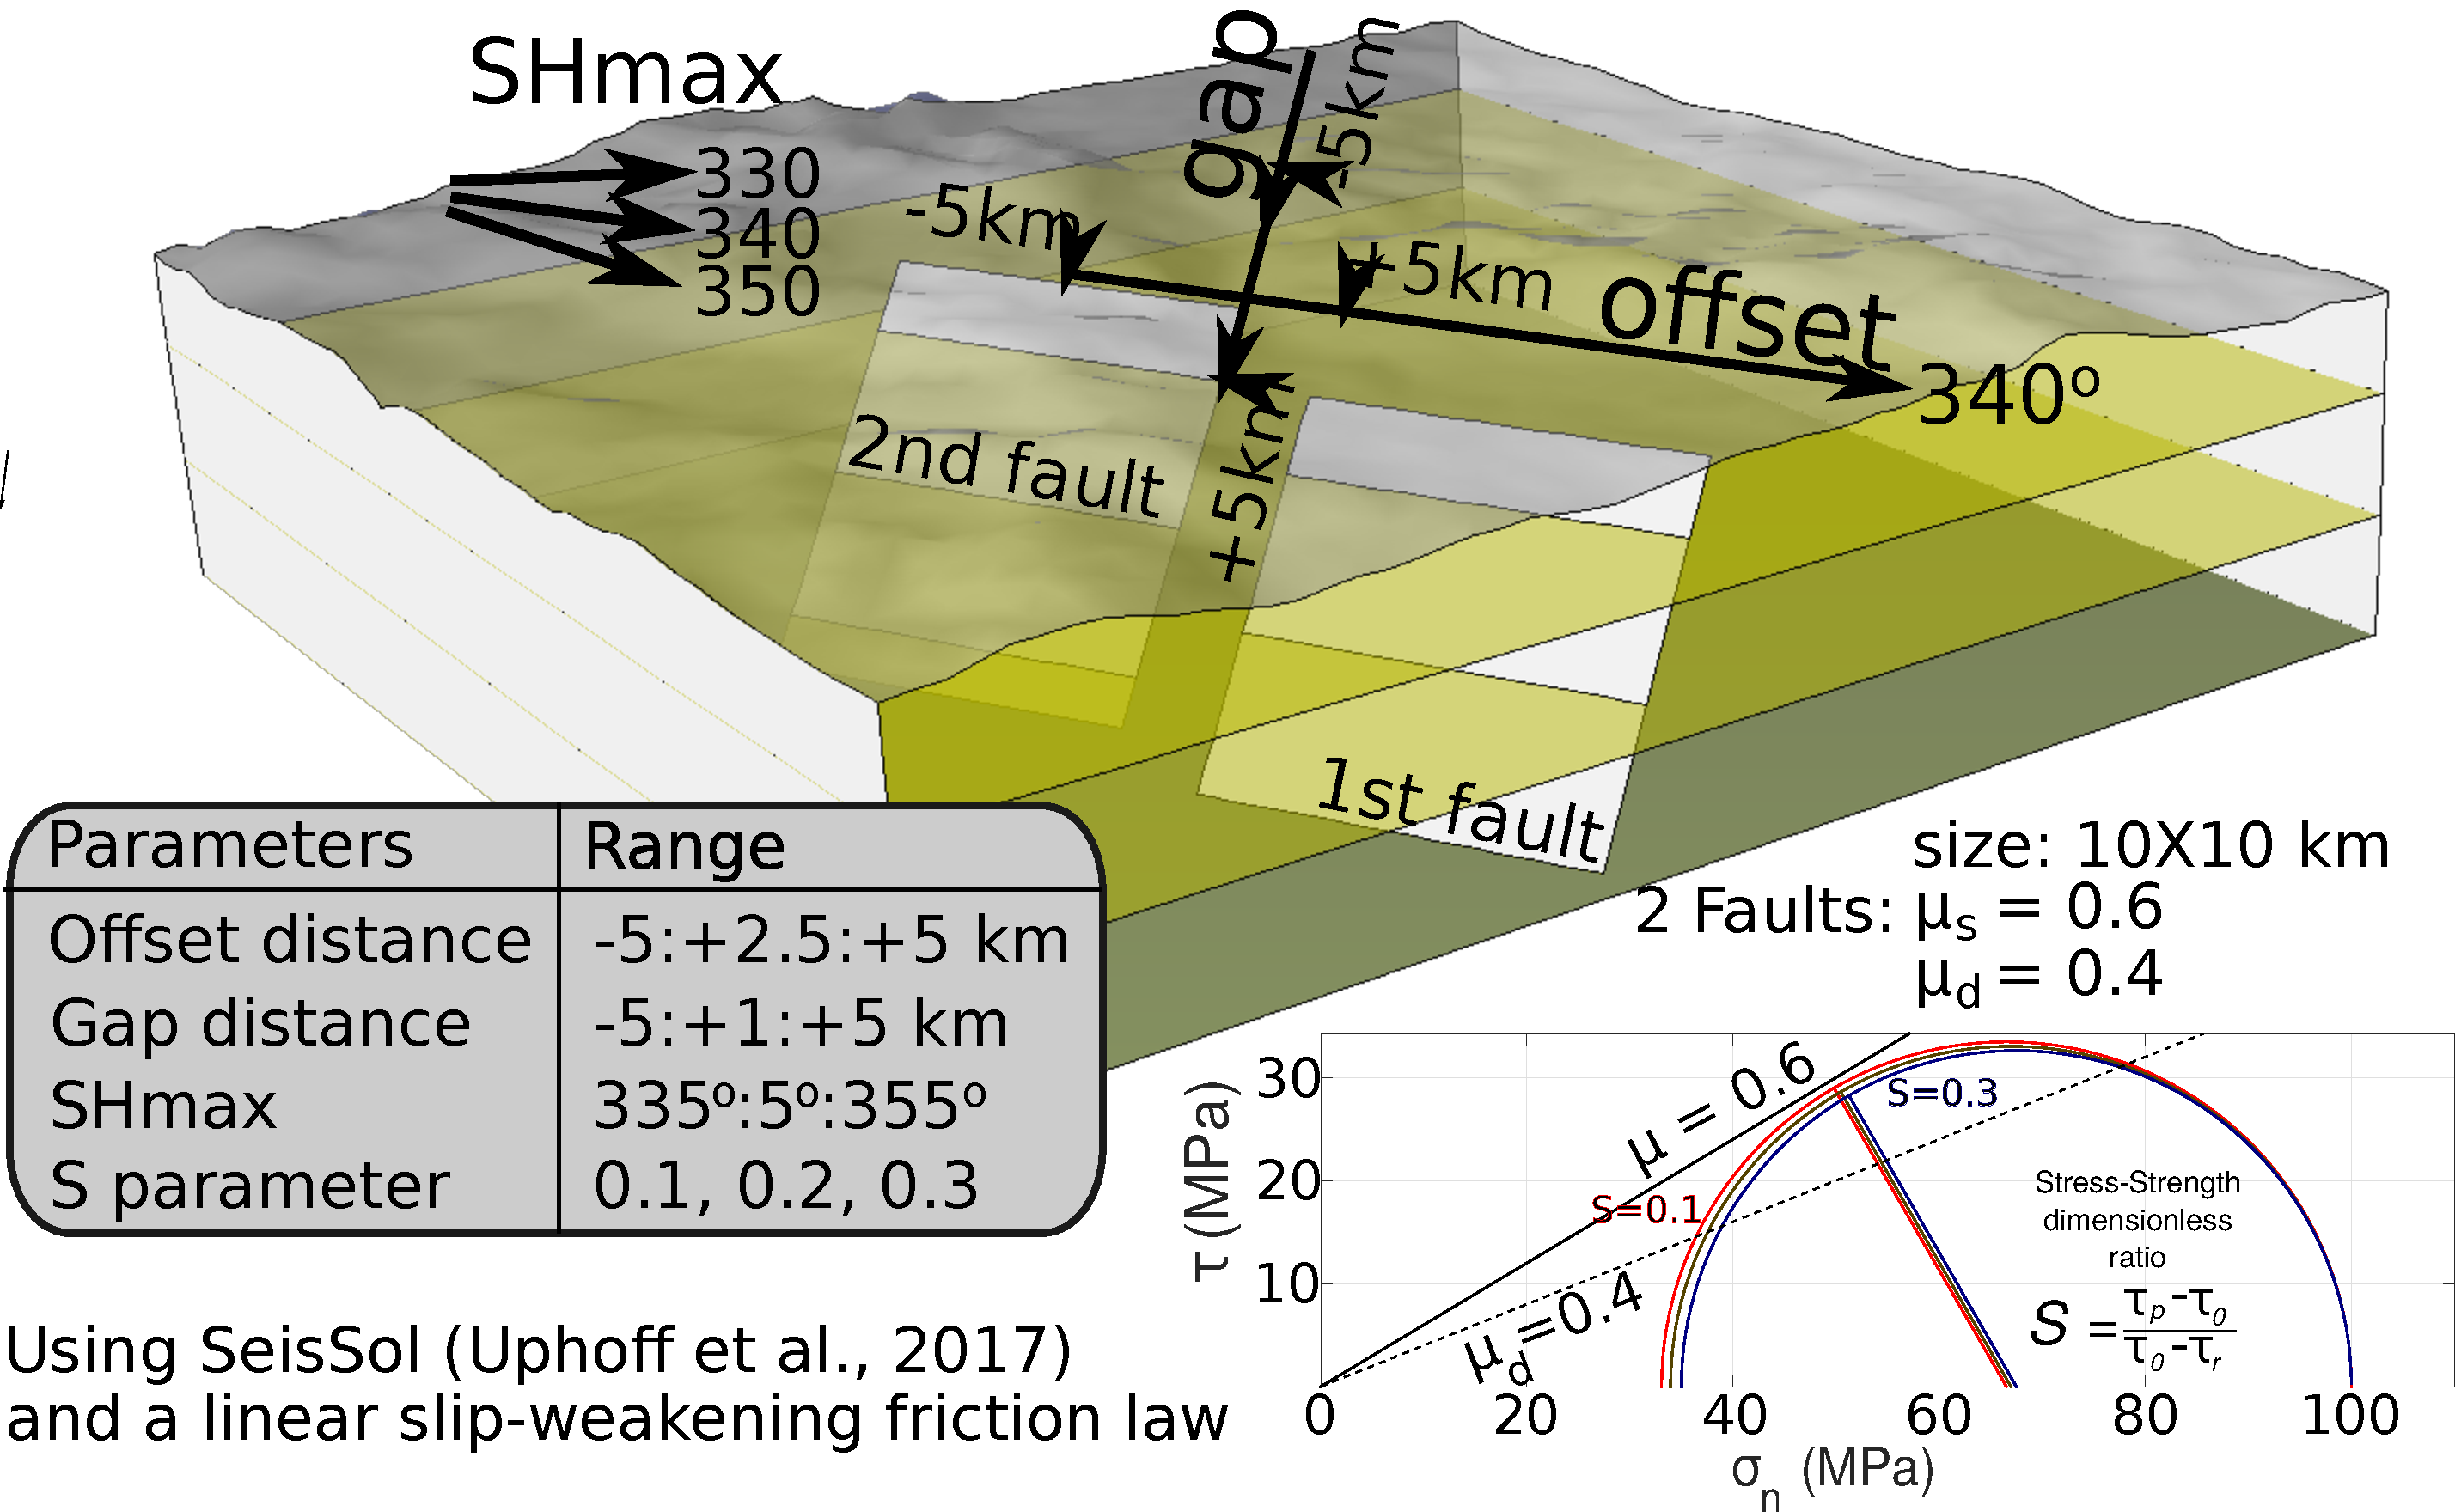
\includegraphics[width=1\linewidth]{images/model.pdf}



}

\headerbox{{\bf 4.} Jump ? How ? When ? Why ?}{name=snaps,column=1,row=0,span=2}{

\begin{minipage}{0.48\linewidth}
 \centering {\bf Fault fixed}
\end{minipage}
\begin{minipage}{0.48\linewidth}
 \centering {\bf Fault not fixed}
\end{minipage}

}


\headerbox{{\bf 3.} Simulation-Results}{name=summary,column=1,row=1,span=1,below=snaps}{

}


\headerbox{{\bf 5.} Results}{name=results,column=2,row=1,span=1,below=snaps}{

}

\headerbox{Refernces}{name=snaps,column=2,row=1,span=1,below=results}{

}



\end{poster}
\end{document}

